\chapter{Background}
\label{background}
This chapter provides the necessary background required to read and understand this report. Section \ref{ad_hoc_network} describes ad hoc networks, their unique characteristics and challenges they might introduce. The chapter then continues to explain how routing is done where two different ad hoc routing protocols are used as examples. The last section \ref{authentication} gives a short overview of different authentication mechanisms common for computer networks.

%\section{Related work}
%Some work has been done previously when it comes to developing and implementing a secure and restricted ad hoc network. Amongst them worth mentioning... blablabla
%Secure Routing for Mobile Ad hoc Networks
%A Performance Comparison of Multi-Hop Wireless Ad Hoc NeWork Routing Protocols
%Secure Extension to the OLSR protocol


\section{Ad Hoc Network}
\label{ad_hoc_network} 
Definition: \textit{``A self-organizing communications network with no form of pre-existing infrastructure or fixed centralized administration.''}
\\\\
A wireless ad hoc network is a collection of nodes able to communicate with each other by together creating and organizing a network. The network is able to perform regular network functions like access and routing without there being any pre-existing, fixed and centralized infrastructure. Thus nodes are not only end-entities, but must also be able to act like a router by forwarding traffic that is not destined to it self. %skriv bedre!
\\\\
The nodes participating in an ad hoc network can either be fixed or mobile. Ad hoc networks where the nodes are mobile, are often referred to as Mobile Ad hoc Networks (MANETs). A closely related variant of the MANET is the mesh network where the nodes are not very mobile or not mobile at all, but they can however still join or leave the network at will making the behavior of the network similar to that of a MANETs. In this report we will focus on ad hoc networks where the participating nodes can be highly mobile, thus when the term ad hoc network or just network is used, we refer to MANET unless otherwise stated.

\subsection{Applications}
\label{ad_hoc_applications}
Because of ad hoc networks self-organizing nature they need very few pre-conditions in place for establishing and maintaining a network. Thus deploying an ad hoc network can be less demanding and very quick compared to other communications network like a traditional computer network \cite{murthy-ad}. Due to ad hoc networks' special characteristics they may find applications in several areas as briefly described below.
\\\\
In emergency situations such as during war or after natural disasters, entire infrastructure-based communication may be destroyed and restoring communication quickly is crucial. By using an ad-hoc network, communication could be set up almost immediately and could then be used in emergency operations such as crowd control, search and rescue, coordinate rescue operations and so on.
\\\\
Military applications also benefit from ad hoc networks ability to form a communication network quickly. In addition to this, military operations usually require a high level of security not only by encrypting the data being transmitted, but also restricting the access to the network.
\\\\
The type of communication required in the environments mentioned above enforces other important requirements on ad hoc networks, such as reliability, efficiency, and support for multicast routing \cite{murthy-ad}. These scenarios will also be covered and further explained in chapter \ref{scenario_requirements}.
\\\\
Other areas of use for ad hoc networks are wireless sensor networks and collaborative and distributed computing \cite{murthy-ad}.

\subsection{Challenges and Issues}
\label{ad_hoc_challenges}
Despite the many of advantages that ad hoc networks may introduce, several challenges and issues are also present that affect the design, deployment, and performance of such networks. Amongst the major issues relevant for our project, we find:
%\cite{misic2008wireless}, \cite{sheu2005handbook} and \cite{murthy-ad}:

\begin{itemize}
\item Mobility of nodes
\item Unreliable medium
\item Resource constraints
\end{itemize}

\noindent
High mobility of nodes in ad hoc networks results in frequent path breaks, packet collisions, transient loops and route flapping. This causes the network topology to change randomly and frequently making it highly dynamic. Hidden and exposed terminal problems may also appear as a consequence of the mobility of the nodes. A good routing protocol should however efficiently solve or reduce the impact of such issues \cite{murthy-ad}.
\\\\
In wireless and especially in noisy wireless areas, data packets can and will get lost. In addition, ad hoc networks with only one wireless communication interface have to cope with self-inflicted interference caused by their own wireless traffic. Thus communication links may have varying quality in terms of packet loss and will therefore also affect the network topology \cite{batman_rfc}.
\\\\
All the issues mentioned above will in turn also affect the security in ad hoc network as explained in the next section.

\subsection{Security Issues}
\label{adhoc_security}
Security in ad hoc networks is a challenging and comprehensive task. The unique characteristics of these networks introduce situations that are not common to traditional computer networks. 
\\\\
Computer networks are infrastructure-based communications networks where there exists important central entities that are necessary in order to have a functional network, e.g. routers, gateways etc. These are points in the network where it is natural to place security mechanisms. However, since ad hoc networks do not have any central entities, there are no well defined points where these mechanisms could be applied \cite{murthy-ad}.
\\\\
Nodes that participate in an ad hoc network can frequently join and leave at any point in time. If there is no authentication mechanism present, there is no association or relationship between nodes and networks making it easy for an intruder to join a network and carry out an attack \cite{murthy-ad}.
\\\\
Unlike wired networks, the communication in wireless ad hoc networks is done on a shared radio channel and may easily be picked up by any node that is in range of direct transmission. A malicious node is therefore able to perform security attacks ranging from passive eavesdropping to active message replay, and message distortion \cite{806983}.
\\\\
Other aspects of ad hoc networks that may affect the security, is the limited resource availability found in such networks. Mobile nodes typically have limited computation capacity, battery power and scarce bandwidth which makes it difficult to implement computation-intensive tasks like complex cryptography-based security mechanisms \cite{1269716}.
\\\\
Different types of security attacks possible in ad hoc networks can be found in all the layers in the OSI model \cite{kurosecomputer}. Some examples of attacks that can be found in the network layer are wormhole, blackhole, Byzantine, information disclosure and routing attacks. On the transport layer we can find attacks like session hijacking. In addition there are attacks which could occur in any layer, such as Denial of Service (DoS) and impersonation \cite{murthy-ad}.

\section{Ad Hoc Routing}\label{ad_hoc_routing}
As explained in \cite{murthy-ad} the responsibilities of a routing protocol include exchanging route information, finding a good path to a destination, discovering dead links, and restoring the paths. 
\\\\
Because of ad hoc networks' unique nature, classical routing protocols are typically not well suited. Thus several routing protocols have over the years been developed specifically for ad hoc networks and they can be categorized into different groups based on their properties.
\\\\
In the sections below, two ad hoc routing protocols will be described and discussed. First out is OLSR which is a common and widely used protocol tailored for ad hoc networks \cite{zafar2008using}. The second routing protocol is BATMAN which was developed as an alternative for OLSR.

\subsection{Optimized Link State Routing protocol}
Optimized Link State Routing protocol (OLSR) is a proactive routing protocol which means that the routing in the network is done based on routing information that is periodically exchanged between nodes. The protocol belongs to the family of classical Link State Protocols which is one of two broad categories of routing protocols used in packet switching networks \cite{clausen2003rfc3626}.
\\\\
OLSR is tailored for mobile ad hoc networks by optimizing the link state protocol in two ways \cite{murthy-ad}: 

\begin{itemize}
\item reducing the size of control packets sent in the network.
\item reducing the number of links that are used for forwarding link state packets.
\end{itemize}

\noindent
These optimizations are realized by using only selected nodes, called Multipoint Relays (MPR), to retransmit control messages and link-state updates sent in the network. Every node in the network, called a Multipoint Relay Selector, chooses a set of neighboring nodes as their MPRs. The protocol uses hop-by-hop routing where only local information is used to route packets. This information is retrieved from the MPRs that periodically announce link-state information and control traffic to their MPR selectors. The basic layout of any packet that is transmitted in OLSR is shown in Figure \ref{fig:olsr}.

\begin{figure}[ht]
	\centering
		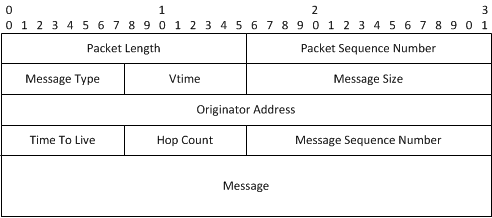
\includegraphics{images/olsr.png}
	\caption{OLSR packet format omitting the IP and UDP headers.}
	\label{fig:olsr}
\end{figure}

\noindent
Because of the regular transmission of control messages, the protocol is sustainable to packet loss which is common in wireless networks. Overhead of control messages in the network is also reduced and redundant control traffic is eliminated by using the MPRs \cite{clausen2003rfc3626}. However, because of the many optimizations added to make the protocol more suitable for ad hoc networks, it also is more complex than e.g. the BATMAN protocol explained in the section below.

\subsection{B.A.T.M.A.N.}\label{batman}
B.A.T.M.A.N., or BATMAN as we will continue to write, is an abbreviation for a "Better Approach To Mobile Ad hoc Networking". It was created with the hope of being a simpler, better and more robust alternative to OLSR. The initial motivation to start the development of the protocol was mainly based on the following reasons \cite{open_mesh}:

\begin{itemize}
\item The OLSR protocol seemed not to be very functional when implemented as specified in \cite{clausen2003rfc3626}. %RFC3626

\item The OLSR protocol depends heavily on the assumption that every node in the network is in possession of almost the same information as all of the other nodes. As they use this information to calculate full routing path to all nodes, the more this information between the nodes differ amongst them, the more likely things like routing loops will occur.
\end{itemize}

\noindent
In order to implement functional OLSR protocol to be used in real-life, the developers found themselves stripping it down removing mechanisms that were initially added to the protocol to optimize it. Eventually the developers had to break compatibility with the protocol defined in \cite{clausen2003rfc3626}. A group of developers felt the OLSR protocol was becoming far to complex and decided develop a routing protocol that was simpler and better, namely BATMAN.
\\\\
BATMAN is, as well as OLSR, a proactive routing protocol where every node has a routing table containing all of the nodes in the network that are accessible via single-hop or multi-hop communication links. The table, which is referred to as Originator List, does however not include the full path to a destination, only the best link-local neighbor towards it. Link-local neighbors are usually referred to as direct neighbors in the BATMAN protocol.
\\\\
Nodes in the BATMAN network build their Originator Lists based on Originator Messages (OGM). These messages are small, containing only a limited amount of information such as version, Time-To-Live (TTL), sequence number, some flags and an Originator Address. The Originator Address is the IP-address of the Originator where the OGM was generated. An Originator is defined in \cite{batman_rfc} as a network interface utilized by BATMAN. Every node in the network periodically generates and broadcasts OGMs for each interface it can communicate through. These messages will be re-broadcasted through the network according to BATMANs forwarding rules until they have reached all the nodes at least once. The format of an OGM is shown in Figure \ref{fig:ogm}.

\begin{figure}[ht]
	\centering
		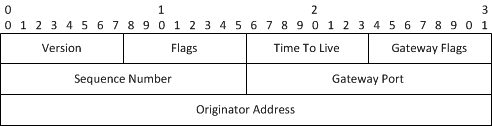
\includegraphics{images/ogm.png}
	\caption{Originator Message (OGM) Format.}
	\label{fig:ogm}
\end{figure}

\noindent
\\\\
The best route to a certain Originator is found by counting the number of OGMs received containing this Originator Address and logging which neighbor it was received from. The best route is thus the link-local neighbor that has the highest count.
\\\\
Details about the BATMAN protocol can be found in the Appendix \ref{appendix_batman}.

\subsection{B.A.T.M.A.N. and OLSR Comparison}\label{batman_olsr_comparison}
One major difference between BATMAN and OLSR is that while OLSR works to reduce the traffic load in the network by restricting which nodes that are allowed to flood, BATMAN does not care about this at all. The reasoning behind this decision is because the protocol was designed to function on unreliable media which is very unstable and can suffer from high packet loss. Thus the flooding of routing information will not saturate the network since most of the packets will be lost due to the lossy media \cite{batman_rfc}.
\\\\
In addition, the nodes in a BATMAN network do not have to calculate the full routing path to all other nodes in the network. By only choosing the next hop towards a destination makes BATMAN a lightweight protocol that quickly adapts to the dynamic topology of ad hoc networks.

\section{Authentication Using Certificates}\label{authentication} % Ny tittel!? authentication and access control / certificates / x.509 certificates
In order to have a restricted ad hoc network there needs to be some form of access control mechanism in place. In traditional computer networks the issue of access control and authentication is usually solved with the use of a hierarchy of trusted third parties, and digital certificates which is associated with every entity participating in the network. A certificate contains information about the entity that defines its identity and rights in the network.
\\\\
This section describes some of the different variants of the X.509 certificates that are used in X.509 Public Key Infrastructure (PKI). 

\subsection{X.509 Long-Lived Public-Key Certificates} \label{LLPKC}
In a Public Key Infrastructure (PKI) the conventional digital certificates are sometimes called Long-Lived Public-key Certificates (LLPKC). They are issued to end-entities by a well-known and trusted Certificate Authority (CA) that digitally signs the certificates with its private key such that it can be verified by anyone in possession of the CAs public key. Each certificate contains the public key of an end-entity and additional data such as subject's public key information, signature algorithm identifier and issuer name \cite{stallings2006cryptography}. 
\\\\
The certificate also contains a validity period of usually months or years which is why they are referred to as "Long-Lived Certificates". This long lifetime entails that a certificate needs to be checked against a Certificate Revocation List (CRL) to ensure that it has not been made invalid whilst still in its validity period. Figure \ref{fig:LLPKC} shows an illustration of a service verifying an end-entity's LLPKC and checking it against a Certificate Revocation List.

\begin{figure}[ht]
	\centering
		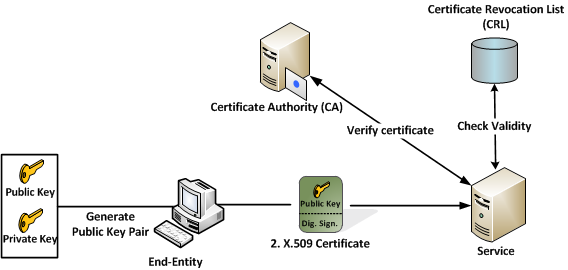
\includegraphics{images/LLPKC.png}
	\caption{An conceptual illustration of the authentication process using LLPKCs.}
	\label{fig:LLPKC}
\end{figure} 

\subsection{X.509 Proxy Certificates} \label{background_pc}
A X.509 Proxy Certificate (PC) is a conventional X.509 public-key certificate containing a critical proxy certificate information extension. The presence of this extension indicates that the certificate is a PC and that it contains one required and two optional fields; pCPathLenConstraint, proxyPolicy and Proxy Certificate Path \cite{tuecke2004rfc3820}.
\\\\
The policy field in the extension can be used to make the PC a Restricted Proxy Certificate (RPC). It contains a field which specifies the appropriate language in which the policy is expressed. This option was intended to provide a finer granularity of control in the rights being delegated.
\\\\
A PC inhabits some of the following properties as described in the Internet standard \cite{tuecke2004rfc3820}:

\begin{itemize}
\item It is signed by an X.509 End Entity Certificate (EEC), or by another PC and is called a Proxy Issuer (PI).
\item An EEC can give certain rights and restrictions to the PC it signs. 
\item It can sign another PC, but nothing else.
\item It contains its own unique public and private key pair.
\item It can be created with any desired lifetime.
\end{itemize}

\noindent
An important feature of the PC is that it is given a unique identity derived from the end-entity who signed it. During the signing the PC may also inherit rights from the PI, subject to the restrictions that are placed on that PC by the PI. Thus the PC has a unique identification which can be used independently and still be associated with the PI who signed the certificate.


\subsection{Other Certificates}
Other variants of the X.509 certificate worth mentioning are Attribute Certificates (AC) and Short-Lived Certificates (SLC). ACs are certificates with a similar structure as a LLPKC, but without a PKC key pair. They contain a set of attributes tied to an identity which is used for authorization and access control decisions. ACs are usually used in association with another certificate that do contain a PKC key pair, such as a LLPKC. The AC may have any validity period desired by the issuer and is usually has a shorter lifetime than LLPKC \cite{farrells2010rfc5755}.
\\\\
The SLCs are modified versions of the traditional X.509 certificates and differ from these mainly because of two characteristics: certificate validity period is no more than 1 million seconds and there is no association between the client and Public Key cryptography (PKC) key pairs \cite{hsu2002intranet}. They were introduced by \cite{hsu2002intranet} with the goal of reducing the costly and difficult key management issues in typical X.509 authentication framework.












